\section{Results}

Figures \ref{fig:cl}, \ref{fig:cd}, and \ref{fig:ld} demonstrate Deflection Theory's efficacy up until stall.

\graphicspath{{./}}

\begin{figure}[htb]
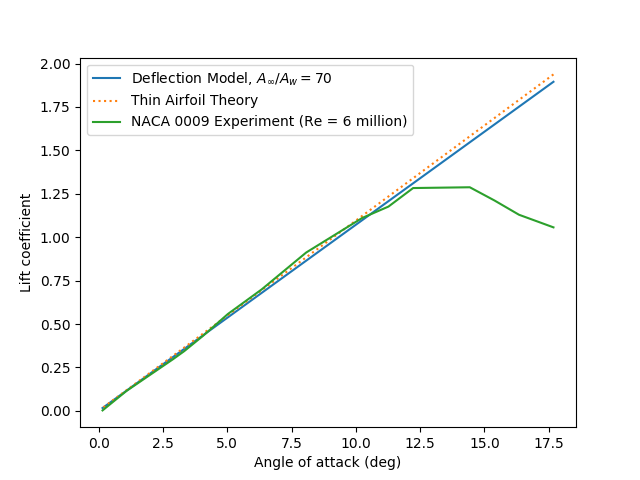
\includegraphics[totalheight=4.5cm]{cl}
\caption{Lift coefficient predictions from Thin Airfoil Theory, the present Deflection Theory, and NACA 0009 experimental data.}
\label{fig:cl}
\end{figure}

\begin{figure}[htb]
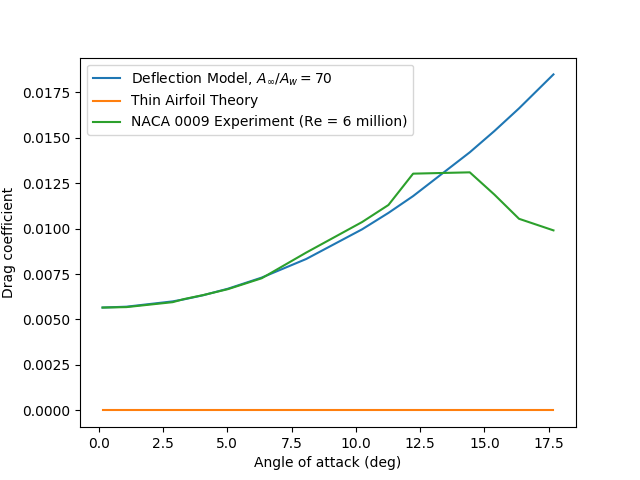
\includegraphics[totalheight=4.5cm]{cd}
\caption{Drag coefficient predictions from Thin Airfoil Theory, the present Deflection Theory, and NACA 0009 experimental data.}
\label{fig:cd}
\end{figure}

\begin{figure}[htb]
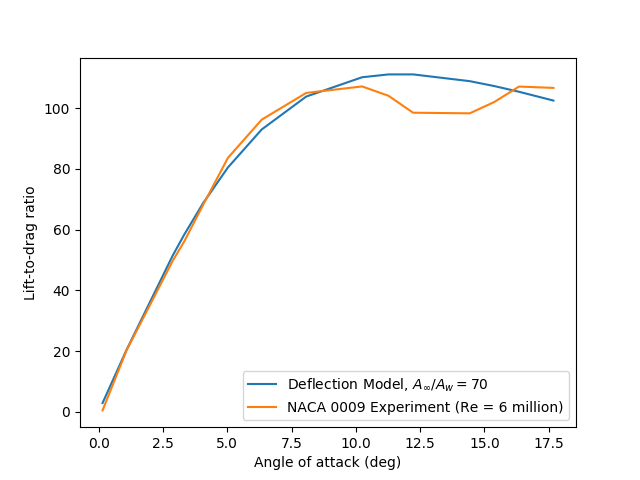
\includegraphics[totalheight=4.5cm]{ld}
\caption{Lift-to-drag ratio predictions from the present Deflection Theory, and NACA 0009 experimental data.}
\label{fig:ld}
\end{figure}

Figures \ref{fig:cl_ratio}, \ref{fig:cd_ratio}, and \ref{fig:ld_ratio} show the sensitivity of performance on \(A_\infty / A_w\).
Lift predictions are much less sensitive to \(A_\infty / A_w\) than the drag predictions are.

\begin{figure}[htb]
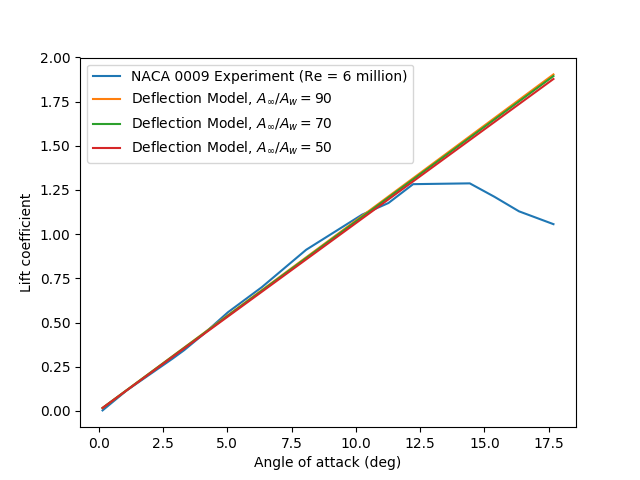
\includegraphics[totalheight=4.5cm]{cl_ratio}
\caption{Sensitivity of Deflection Theory lift predictions to the \(A_\infty / A_w\) parameter.}
\label{fig:cl_ratio}
\end{figure}

\begin{figure}[htb]
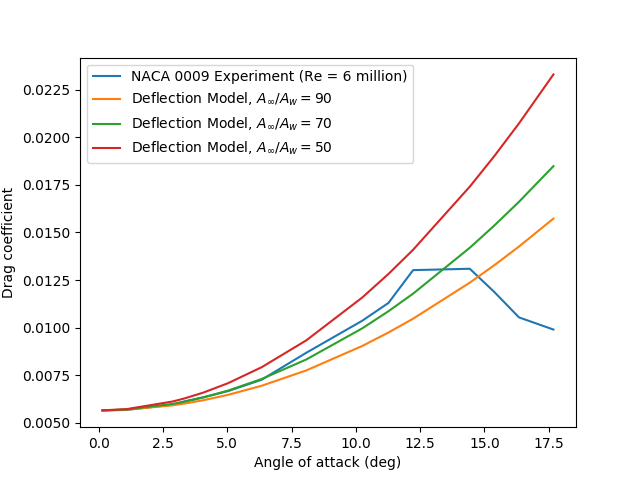
\includegraphics[totalheight=4.5cm]{cd_ratio}
\caption{Sensitivity of Deflection Theory drag predictions to the \(A_\infty / A_w\) parameter.}
\label{fig:cd_ratio}
\end{figure}

\begin{figure}[htb]
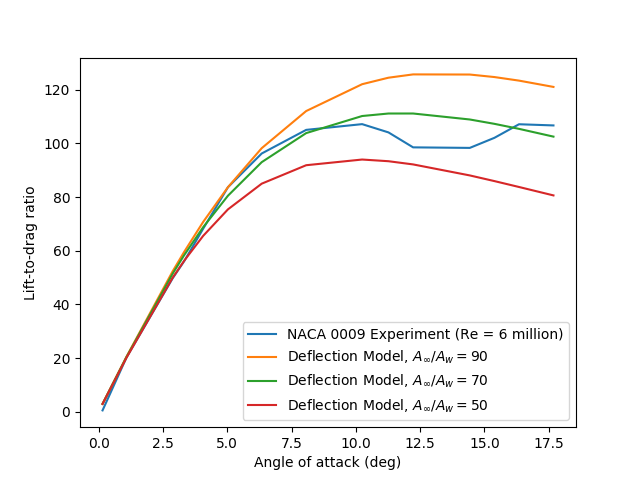
\includegraphics[totalheight=4.5cm]{ld_ratio}
\caption{Sensitivity of Deflection Theory lift-to-drag ratio predictions to the \(A_\infty / A_w\) parameter.}
\label{fig:ld_ratio}
\end{figure}

